\documentclass{beamer}

\mode<presentation>

\usetheme{Montpellier}

% \usepackage{url}
\usepackage[utf8]{inputenc}
\usepackage[ngerman]{babel}
\usepackage{amsfonts,amsmath,amssymb}
\usepackage{graphicx}
\usepackage{textcomp}
\usepackage{epstopdf}
\usepackage{lmodern}
\usepackage[T1]{fontenc}
\usepackage{todonotes}
\let\todox\todo
\renewcommand\todo[1]{\todox[inline]{#1}}

% \setcounter{tocdepth}{2}

\title{\LaTeX-Einführung}
\author{Florian Uekermann und Julian Cambeis\newline Überarbeitet von Jakob Borchardt \newline Überarbeitet von Yannik Schädler}
\date{\today}

\begin{document}

\begin{frame}
  \titlepage
\end{frame}

\section{Wozu \LaTeX?}
\begin{frame}
  \frametitle{Wozu \LaTeX?}
    \begin{itemize}
      \item<1-> Zeit- und Stressersparnis
      \item<2-> Plattformunabhängig
      \item<3-> kostenlos
      \item<4-> gut dokumentiert (Internet, Bücher)
      \item<5-> Quasistandard bei wissenschaftlichen Veröffentlichungen
    \end{itemize}
\end{frame}

\section{Bevor wir anfangen}
\begin{frame}
\frametitle{Bevor wir anfangen}
  \begin{itemize}
    \item<1-> Einen Ordner "`\LaTeX"' erstellen
    \item<2-> jedes Dokument in eigenem Ordner
    \item<3-> Neues Dokument im Editor öffnen und im neuen Ordner speichern
    \item<4-> logisches Einrücken macht eure Datei übersichtlich
  \end{itemize}
\end{frame}

\section{Dokumentstruktur}
\subsection{Der Kopf (Header)}
\begin{frame}
 \begin{center}
  \Huge Dokumentenstruktur \\
  \Large Der Kopf (Header)
 \end{center}
\end{frame}

\begin{frame}[fragile]
\frametitle{Dokumentstruktur}
\framesubtitle{Der Kopf (Header)}
\begin{semiverbatim}
 \uncover<1->{\small \\documentclass[a4paper,11pt,DIV=11,parskip=half*]\{scrartcl\} \normalsize}
 \uncover<2->{\\usepackage[utf8]\{inputenc\}}
 \uncover<3->{\\usepackage[ngerman]\{babel\}}
 \uncover<4->{\\usepackage\{amsfonts, amsmath, amssymb\}}
 \uncover<4->{}
 \uncover<5->{\\title\{Der Title\}}
 \uncover<6->{\\author\{Mein Name\}}
 \uncover<7->{\\date\{Datum oder \\today\}}
\end{semiverbatim}
\end{frame}


\subsection{Der Hauptteil (Dokument}
\begin{frame}
 \begin{center}
  \Huge Dokumentenstruktur \\
  \Large Der Hauptteil (Dokument)
 \end{center}
\end{frame}

\begin{frame}[fragile]
\frametitle{Dokumentstruktur}
\framesubtitle{Der Hauptteil (Dokument)}
  \setbeamercolor{alerted text}{fg=blue}
  \setbeamerfont{alerted text}{series=\bfseries,family=\ttfamily}
  \begin{semiverbatim}
    \uncover<1->{\\begin\{document\}}
    \uncover<1->{}
    \uncover<2->{  \\maketitle}
    \uncover<1->{}
    \uncover<3->{    \\section\{Integration \\& Differentiation\}}
    \uncover<3->{    Wichtige Regeln für Integration und}
    \uncover<3->{    Differentiation}
    \uncover<3->{}
    \uncover<4->{    \\section\{Additionstheoreme\}}
    \uncover<4->{    Wichtige Additionstheoreme}
    \uncover<1->{}
    \uncover<1->{\\end\{document\}}
  \end{semiverbatim}
\end{frame}

\subsection{Einfaches Dokument}
\begin{frame}
 \frametitle{Einfaches Dokument - Ergebnis}
  \begin{center}
  \huge \textbf{Der Titel}\\
  \vspace{1ex}
  \normalsize Mein Name\\
  \vspace{1ex}
  Datum oder 18. April 2013\\
%   \includegraphics[width=0.9\textwidth]{einfdok.eps}
  \end{center}
\textbf{1 Integration \& Differentiation}\\
\vspace{1ex}
\scriptsize Wichtige Regeln für Integration und Differentiation\\
\vspace{1.5ex}
\normalsize \textbf{2 Additionstheoreme}\\
% \vspace{0.5ex}
\scriptsize Wichtige Additionstheoreme
\end{frame}


\section{Textformatierung}
\begin{frame}
 \begin{center}
  \Huge Textformatierung
 \end{center}
\end{frame}

\subsection{Textformatierung - fett usw.}
\begin{frame}[fragile]
  \begin{tabular}{ ll }
		\uncover<1->{Zeilenumbruch:} & \begin{minipage}{3in}\begin{semiverbatim}\uncover<1->{\\\\}\end{semiverbatim}\end{minipage} \\ & \\
    \uncover<2->{ein Text} & \begin{minipage}{3in}\begin{semiverbatim}\uncover<2->{ein Text}\end{semiverbatim}\end{minipage}\\ & \\
    \uncover<3->{\textbf{fetter Text}} & \begin{minipage}{3in}\begin{semiverbatim}\uncover<3->{\\textbf\{fetter Text\}}\end{semiverbatim}\end{minipage}\\ & \\
    \uncover<4->{\textit{kursiver Text}} & \begin{minipage}{3in}\begin{semiverbatim}\uncover<4->{\\textit\{kursiver Text\}}\end{semiverbatim}\end{minipage}\\ & \\
    \uncover<5->{\underline{unterstrichener Text}} & \begin{minipage}{3in}\begin{semiverbatim}\uncover<5->{\\underline\{unterstrichener Text\}}\end{semiverbatim}\end{minipage}\\ & \\
    \uncover<6->{\texttt{Schreibmaschinentext}} & \begin{minipage}{3in}\begin{semiverbatim}\uncover<6->{\\texttt\{Schreibmaschinentext\}}\end{semiverbatim}\end{minipage}\\ & \\
    \uncover<7->{\underline{\textbf{Text}}} & \begin{minipage}{3in}\begin{semiverbatim}\uncover<7->{\\underline\{\\textbf\{Text\}\}}\end{semiverbatim}\end{minipage}
 \end{tabular}
\end{frame}

\subsection{Textformatierung - Schriftgrößen}
\begin{frame}[fragile]
  \uncover<2->{\Large Ein teilweise groß \normalsize geschriebener Satz.}
  \begin{semiverbatim}\uncover<1->{\alert<1-2>{\\Large} Ein teilweise groß \alert<1-2>{\\normalsize}}
  \uncover<1->{geschriebener Satz.}\end{semiverbatim}
  \uncover<4->{\tiny Wichtige \scriptsize Befehle \footnotesize für \small Schriftgrößen}
  \uncover<4->{\normalsize die \large ihr \Large immer \huge wieder \Huge benutzen \normalsize könnt.}
  \begin{semiverbatim}
  \uncover<3->{\alert<3-4>{\\tiny} Wichtige \alert<3-4>{\\scriptsize} Befehle \alert<3-4>{\\footnotesize}}
  \uncover<3->{für \alert<3-4>{\\small} Schriftgrößen \alert<3-4>{\\normalsize} die \alert<3-4>{\\large}}
  \uncover<3->{ihr \alert<3-4>{\\Large} immer \alert<3-4>{\\huge} wieder \alert<3-4>{\\Huge}}
  \uncover<3->{benutzen \alert<3-4>{\\normalsize} könnt.}
  \end{semiverbatim}
\end{frame}

\subsection{Textformatierung - Unterkapitel}
\begin{frame}[fragile]
\frametitle{Unterkapitel}
\begin{semiverbatim}
  \uncover<1->{\\section\{Integration \\& Differentiation\}}
  \uncover<1->{  Wichtige Regeln für Integration und}
  \uncover<1->{  Differentiation}
  \uncover<1->{}
  \uncover<2->{  \\subsection\{Differentiation\}}
  \uncover<1->{}
  \uncover<3->{    \\subsubsection\{Produktregel\}}
  \uncover<3->{    Die Produktregel}
  \uncover<1->{}
  \uncover<3->{    \\subsubsection\{Kettenregel\}}
  \uncover<3->{    Die Kettenregel}
  \uncover<1->{}
  \uncover<2->{  \\subsection\{Integration\}}
  \uncover<2->{  Integrationsregeln}
\end{semiverbatim}
\end{frame}

\begin{frame}
\frametitle{Unterkapitel - Ergebnis}
  \Large \textbf{1 Integration \& Differentiation} \\
  \vspace{1ex}
  \normalsize Wichtige Regeln für Integration und Differentiation\\
  \vspace{2ex}
  \large \textbf{1.1 Differentiation} \\
  \vspace{1ex}
  \normalsize \textbf{1.1.1 Produktregel} \\
  Die Produktregel\\
  \vspace{2ex}
  \textbf{1.1.2 Kettenregel} \\
  Die Kettenregel \\
  \vspace{2ex}
  \large \textbf{1.2 Integration}\\
  \vspace{1ex}
  \normalsize Integrationsregeln
\end{frame}

\subsection{Textformatierung - Unterkapitel}
\begin{frame}[fragile]
\frametitle{Unterkapitel}
\begin{semiverbatim}
  \uncover<1->{\\section\{Integration \\& Differentiation\}}
  \uncover<1->{  Wichtige Regeln für Integration und}
  \uncover<1->{  Differentiation}
  \uncover<1->{}
  \uncover<1->{  \\subsection\{Differentiation\}}
  \uncover<1->{}
  \uncover<2->{    \\subsubsection\alert<2>{*}\{Produktregel\}}
  \uncover<2->{    Die Produktregel}
  \uncover<1->{}
  \uncover<2->{    \\subsubsection\alert<2>{*}\{Kettenregel\}}
  \uncover<2->{    Die Kettenregel}
  \uncover<1->{}
  \uncover<1->{  \\subsection\{Integration\}}
  \uncover<1->{  Integrationsregeln}
\end{semiverbatim}
\end{frame}

\begin{frame}
\frametitle{Unterkapitel - Ergebnis}
  \Large \textbf{1 Integration \& Differentiation} \\
  \vspace{1ex}
  \normalsize Wichtige Regeln für Integration und Differentiation\\
  \vspace{2ex}
  \large \textbf{1.1 Differentiation} \\
  \vspace{1ex}
  \normalsize \textbf{Produktregel} \\
  Die Produktregel\\
  \vspace{2ex}
  \textbf{Kettenregel} \\
  Die Kettenregel \\
  \vspace{2ex}
  \large \textbf{1.2 Integration}\\
  \vspace{1ex}
  \normalsize Integrationsregeln
\end{frame}

\subsection{Inhaltsverzeichnis}
\begin{frame}[fragile]
\frametitle{Inhaltsverzeichnis}
Inhaltsverzeichnis kann überall erstellt werden, es empfielt sich allerdings am Anfang nach \verb+\maketitle+ .
  \begin{semiverbatim}
    \uncover<1->{\\tableofcontents}
  \end{semiverbatim}
  \uncover<2->{%
    \begin{figure}
      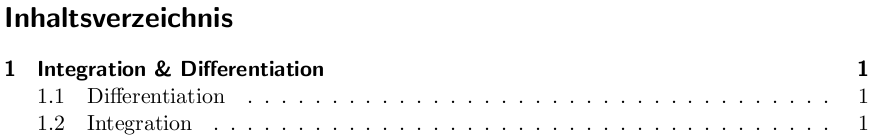
\includegraphics[width=\textwidth]{inhaltsverz.png}
    \end{figure}}
\end{frame}


\subsection{Textformatierung - Anhang}
\begin{frame}[fragile]
\frametitle{Anhang}
  \begin{semiverbatim}
    \uncover<1->{  \\section\{Additionstheoreme\}}
    \uncover<1->{    \\subsection\{Sinus und Cosinus\}}
    \uncover<1->{      Sinus und Cosinus-Funktion}
    \uncover<1->{}
    \uncover<2->{  \\appendix}
    \uncover<1->{}
    \uncover<3->{  \\section\{Quellenverzeichnis\}}
    \uncover<3->{    \\subsection\{Bücher\}}
    \uncover<3->{      Buch 1}
    \uncover<1->{}
    \uncover<3->{  \\section\{Bilder\}}
    \uncover<3->{    \\subsection\{Graphen\}}
    \uncover<3->{      Bilder}
  \end{semiverbatim}
\end{frame}

\begin{frame}
\frametitle{Anhang - Ergebnis}
  \Large \textbf{2 Additionstheoreme} \\
  \vspace{1ex}
  \large \textbf{2.1 Sinus und Cosinus} \\
  \vspace{1ex}
  \normalsize Sinus und Cosinus-Funktion \\
  \vspace{2ex}
  \Large \textbf{A Quellenverzeichnis}\\
  \vspace{1ex}
  \large \textbf{A.1 Bücher} \\
  \vspace{1ex}
  \normalsize Buch 1 \\
  \vspace{2ex}
  \Large \textbf{B Bilder} \\
  \vspace{1ex}
  \large \textbf{B.1 Graphen} \\
  \vspace{1ex}
  \normalsize Bilder
\end{frame}


\begin{frame}
 \begin{center}
  \Huge Listen und Aufzählungen
 \end{center}
\end{frame}

\subsection{Textformatierung - Auflistungen}
\begin{frame}[fragile]
\frametitle{Auflistungen}
  \begin{semiverbatim}
    \uncover<1->{\\begin\{itemize\}}
    \uncover<2->{  \\item Erstes Listenelement}
    \uncover<2->{  \\item Zweites Listenelement}
    \uncover<2->{  \\item Drittes Listenelement}
    \uncover<1->{\\end\{itemize\}}
  \end{semiverbatim}
\uncover<3->{\begin{itemize}
              \item Erstes Listenelement
              \item Zweites Listenelement
              \item Drittes Listenelement
             \end{itemize}}
\end{frame}

\subsection{Textformatierung - Aufzählungen}
\begin{frame}[fragile]
\frametitle{Aufzählungen}
  \begin{semiverbatim}
    \uncover<1->{\\begin\{enumerate\}}
    \uncover<2->{  \\item Erstes Listenelement}
    \uncover<2->{  \\item Zweites Listenelement}
    \uncover<2->{  \\item Drittes Listenelement}
    \uncover<1->{\\end\{enumerate\}}
  \end{semiverbatim}
\uncover<3->{\begin{enumerate}
              \item Erstes Listenelement
              \item Zweites Listenelement
              \item Drittes Listenelement
             \end{enumerate}}
\end{frame}

\subsection{Textformatierung - Eigene Symbole}
\begin{frame}[fragile]
\frametitle{Aufzählungen - Eigene Symbole}
  \begin{semiverbatim}
    \uncover<1->{\\begin\{itemize\}}
    \uncover<2->{  \\item\alert<2>{[1tens]} Erstes Listenelement}
    \uncover<2->{  \\item\alert<2>{[2tens]} Zweites Listenelement}
    \uncover<2->{  \\item\alert<2>{[3tens]} Drittes Listenelement}
    \uncover<1->{\\end\{itemize\}}
  \end{semiverbatim}
\uncover<3->{\begin{itemize}
              \item[1tens] Erstes Listenelement
              \item[2tens] Zweites Listenelement
              \item[3tens] Drittes Listenelement
             \end{itemize}}
\end{frame}


\section{Mathematischer Modus}
\begin{frame}
 \begin{center}
  \Huge Mathematischer Modus \\
  \Large Grundlegende Befehle
 \end{center}
\end{frame}

\subsection{Grundlegende Befehle}
\begin{frame}[fragile]
 \frametitle{Mathematischer Modus - Grundlagen}
	\begin{semiverbatim}
	 \uncover<1->{Eine Formel: \alert<1>{\\(}a=b-c\alert<1>{\\)}}
	\end{semiverbatim}
	\uncover<1->{Eine Formel: \(a=b-c\)}
	\begin{semiverbatim}
	 \uncover<2->{\\(a\alert<2>{^}2+b\alert<2>{^}2=c\alert<2>{^}2\\) ist der Satz des Pythagoras.}
	\end{semiverbatim}
	\uncover<2->{\(a^2+b^2=c^2\) ist der Satz des Pythagoras.}
	\begin{semiverbatim}
	 \uncover<3->{\\(\alert<3>{\\sqrt\{x_1\}}=x_2\\)}
	\end{semiverbatim}
	\uncover<3->{\(\sqrt{x_1}=x_2\)}
	\begin{semiverbatim}
	 \uncover<4->{\\(\alert<4>{\\frac\{a+b\}\{ab\}}\\)}
	\end{semiverbatim}
	\uncover<4->{\(\frac{a+b}{ab}\)}
\end{frame}

\begin{frame}[fragile]
 \frametitle{Mathematischer Modus - Grundlagen}
	\begin{semiverbatim}
	 \uncover<1->{\\(\alert<1>{\\sin \\alpha} = \\frac\{a\}\{c\}\\)}
	\end{semiverbatim}
	\uncover<1->{\(\sin \alpha = \frac{a}{c}\)}
	\begin{semiverbatim}
	 \uncover<2->{\\(\alert<2>{\\delta \\neq \\Delta}\\)}
	\end{semiverbatim}
	\uncover<2->{\(\delta \neq \Delta\)}
	\begin{semiverbatim}
	 \uncover<3->{\\(\\phi \alert<3>{\\cdot} \\varphi = ?\\)}
	\end{semiverbatim}
	\uncover<3->{\(\phi \cdot \varphi = ?\)}
	\begin{semiverbatim}
	 \uncover<4->{\\(\\frac\{\alert<4>{\\text\{Zähler\}}\}\{\alert<4>{\\text\{Nenner\}}\}\\)}
	\end{semiverbatim}
	\uncover<4->{\(\frac{\text{Zähler}}{\text{Nenner}}\)}
\end{frame}

\subsection{Absatz}
\begin{frame}[fragile]
\frametitle{Mathematischer Modus - Absatz}
  \begin{semiverbatim}
    \uncover<1->{Ein Absatz über der Gleichung}
    \uncover<1->{}
    \uncover<1->{\alert<1>{\\[} \\pi \\approx 3\alert<1>{\\]}}
    \uncover<1->{}
    \uncover<1->{Ein Absatz unter der Gleichung}
  \end{semiverbatim}
Ein Absatz über der Gleichung
\[\pi \approx 3\]
Ein Absatz unter der Gleichung
\end{frame}

\begin{frame}
 \begin{center}
  \Huge Mathematischer Modus \\
  \Large Align-Umgebung
 \end{center}
\end{frame}

\subsection{align-Umgebung}
\begin{frame}[fragile]
\frametitle{Die Align-Umgebung}
  \begin{semiverbatim}
    \uncover<1->{\\begin\{align\}}
    \uncover<2->{  \\pi \\approx 3 \alert<2>{\\\\}}
    \uncover<2->{  e = \\exp\{(1)\} \\approx 2 + 1 \alert<2>{\\\\}}
    \uncover<2->{  \\Rightarrow e \\approx \\pi}
    \uncover<1->{\\end\{align\}}
  \end{semiverbatim}
\uncover<3->{%
	    \begin{align}
		\pi \approx 3 \\
		e = \exp{(1)} \approx 2 + 1 \\
		\Rightarrow e \approx \pi
	    \end{align}}
\end{frame}

\begin{frame}[fragile]
\frametitle{Die Align-Umgebung unnumeriert}
 \begin{semiverbatim}
  \uncover<1->{\\begin\{align\alert<1>{*}\}}
  \uncover<1->{  F = m \\cdot a}
  \uncover<1->{\\end\{align\alert<1>{*}\}}
 \end{semiverbatim}
 \uncover<2->{%
	\begin{align*}
	 F = m \cdot a
	\end{align*}}
\end{frame}

\begin{frame}[fragile]
\frametitle{Die Align-Umgebung unnumeriert - 2}
 \begin{semiverbatim}
  \uncover<1->{\\begin\{align\}}
  \uncover<1->{  x = v \\cdot t \alert<1>{\\notag} \\\\}
  \uncover<1->{  \\rightarrow t = \\frac\{x\}\{v\}}
  \uncover<1->{\\end\{align\}}
 \end{semiverbatim}
 \uncover<2->{%
	\begin{align}
	 x &= v \cdot t \notag \\
	 \rightarrow t &= \frac{x}{v}
	\end{align}}
\end{frame}


\begin{frame}[fragile]
\frametitle{Die Align-Umgebung ordnen}
  \begin{semiverbatim}
    \uncover<1->{\\begin\{align\}}
    \uncover<1->{  \\pi \alert<1>{&}\\approx 3 \\\\}
    \uncover<1->{  e = \\exp\{(1)\} \alert<1>{&}\\approx 2 + 1 \\\\}
    \uncover<1->{  \\Rightarrow e \alert<1>{&}\\approx \\pi}
    \uncover<1->{\\end\{align\}}
  \end{semiverbatim}
\uncover<2->{\begin{align}
		\pi &\alert<2>{\approx} 3 \\
		e = \exp{(1)} &\alert<2>{\approx} 2 + 1 \\
		\Rightarrow e &\alert<2>{\approx} \pi
             \end{align}}
\end{frame}

\begin{frame}[fragile]
\frametitle{Die Align-Umgebung ordnen 2}
  \begin{semiverbatim}
    \uncover<1->{\\begin\{align\}}
    \uncover<1->{  \alert<1>{&}\\pi \\approx 3 \\\\}
    \uncover<1->{  \alert<1>{&}e = \\exp\{(1)\} \\approx 2 + 1 \\\\}
    \uncover<1->{  \alert<1>{&}\\Rightarrow e \\approx \\pi}
    \uncover<1->{\\end\{align\}}
  \end{semiverbatim}
\uncover<2->{\begin{align}
		&\pi \approx 3 \\
		&e = \exp{(1)} \approx 2 + 1 \\
		&\Rightarrow e \approx \pi
             \end{align}}
\end{frame}

\begin{frame}
 \begin{center}
  \Huge Mathematischer Modus \\
  \Large Gleichungssysteme
 \end{center}
\end{frame}

\subsection{Gleichungssystem}
\begin{frame}[fragile]
\frametitle{Align-Umgebung - Gleichungssystem}
  \begin{semiverbatim}
    \uncover<1->{\\begin\{align*\}}
    \uncover<1->{  -\alert<1>{&}x \alert<1>{&}+\alert<1>{&}y  \alert<1>{&}+\alert<1>{&}z  \alert<1>{&}= \alert<1>{&}0 \\\\}
    \uncover<1->{  \alert<1>{&}x  \alert<1>{&}-3\alert<1>{&}y \alert<1>{&}-2\alert<1>{&}z \alert<1>{&}= \alert<1>{&}5 \\\\}
    \uncover<1->{  5\alert<1>{&}x \alert<1>{&}+\alert<1>{&}y  \alert<1>{&}+4\alert<1>{&}z \alert<1>{&}= \alert<1>{&}3}
    \uncover<1->{\\end\{align*\}}
  \end{semiverbatim}
  \uncover<2->{%
    \begin{align*}
      -&x &+&y  &+&z  &= &0 \\
      &x  &-3&y &-2&z &= &5 \\
      5&x &+&y  &+4&z &= &3
    \end{align*}}
\end{frame}

\begin{frame}[fragile]
\frametitle{Align-Umgebung - Gleichungssystem}
  \begin{semiverbatim}
    \uncover<1->{\\begin\{align*\}}
    \uncover<1->{  -&x &&+ &&y  &&+ &&z  &&= &&0 \\\\}
    \uncover<1->{  &x  &&- &3&y &&- &2&z &&= &&5 \\\\}
    \uncover<1->{  5&x &&+ &&y  &&+ &4&z &&= &&3}
    \uncover<1->{\\end\{align*\}}
  \end{semiverbatim}
  \uncover<2->{%
    \begin{align*}
      -&x &&+ &&y  &&+ &&z  &&= &&0 \\
      &x  &&- &3&y &&- &2&z &&= &&5 \\
      5&x &&+ &&y  &&+ &4&z &&= &&3
    \end{align*}}
\end{frame}

\begin{frame}
 \begin{center}
  \Huge Mathematischer Modus \\
  \Large Kleinere Tricks
 \end{center}
\end{frame}

\subsection{Matrizen}
\begin{frame}[fragile]
\frametitle{Matrizen}
  \begin{semiverbatim}
    \uncover<1->{\\begin\{align\}}
    \uncover<1->{  \\begin\{pmatrix\}}
    \uncover<2->{    a \alert<2>{&} b \alert<2>{&} c \alert<2>{\\\\}}
    \uncover<2->{    d \alert<2>{&} e \alert<2>{&} f \alert<2>{\\\\}}
    \uncover<2->{    g \alert<2>{&} h \alert<2>{&} i \alert<2>{\\\\}}
    \uncover<2->{    j \alert<2>{&} k \alert<2>{&} l}
    \uncover<1->{  \\end\{pmatrix\}}
    \uncover<1->{\\end\{align\}}
  \end{semiverbatim}
  \uncover<3->{%
    \begin{align}
      \begin{pmatrix}
	a & b & c \\
	d & e & f \\
	g & h & i \\
	j & k & l
      \end{pmatrix}
    \end{align}}
\end{frame}

\subsection{Doppelbrüche}
\begin{frame}[fragile]
\frametitle{Doppelbrüche}
  \begin{semiverbatim}
		\uncover<1->{Normale Doppelbrüche:}
    \uncover<1->{\\(\\frac\{ab\}\{c\} = \\frac\{a\}\{\alert<1>{\\frac\{c\}\{b\}}\}\\)}
    \uncover<1->{\(\frac{ab}{c} = \frac{a}{\frac{c}{b}}\)}
    \uncover<1->{}
    \uncover<2->{Alle Zeichen gleich groß:}
    \uncover<2->{\\(\alert<2>{\\dfrac}\{ab\}\{c\} = \alert<2>{\\dfrac}\{a\}\{\alert<2>{\\dfrac}\{c\}\{b\}\}\\)}
    \uncover<2->{\(\dfrac{ab}{c} = \dfrac{a}{\dfrac{c}{b}}\)}
  \end{semiverbatim}
\end{frame}

\begin{frame}
 \begin{center}
  \Large \uncover<1>{Gibt es Fragen?} \\
  \uncover<2>{Das war's für heute - morgen geht's weiter}
 \end{center}
\end{frame}


\section{Tabellen}
\begin{frame}
 \begin{center}
  \Huge Tabellen
 \end{center}
\end{frame}

\subsection{Grundlage}
\begin{frame}[fragile]
\frametitle{Tabellen}
  \begin{semiverbatim}
    \uncover<1->{\\begin\{tabular\}\alert<2>{\{|l|c|r|\}}}
    \uncover<1->{  \alert<4>{\\hline}}
    \uncover<1->{  Tabelle \alert<3>{&} mit \alert<3>{&} drei Spalten \\\\ \alert<4>{\\hline}}
    \uncover<1->{  aber \alert<3>{&} nur mit zwei \alert<3>{&} Zeilen \\\\ \alert<4>{\\hline}}
    \uncover<1->{\\end\{tabular\}}
  \end{semiverbatim}
  \uncover<5->{%
    \begin{tabular}{|l|c|r|}\hline
      Tabelle & mit & drei Spalten \\\hline
      aber & nur mit zwei & Zeilen \\\hline
    \end{tabular}}
\end{frame}

\begin{frame}[fragile]
\frametitle{Tabellen}
  \begin{semiverbatim}
    \uncover<1->{\\begin\{tabular\}\{|c|\alert<1>{p\{2cm\}}|\alert<1>{p\{4cm\}}\}}
    \uncover<1->{  1. S. & 2. S. mit 2cm & 3. S. mit 4cm}
    \uncover<1->{\\end\{tabular\}}
  \end{semiverbatim}
  \uncover<2->{%
    \begin{tabular}{|c|p{2cm}|p{4cm}}
      1. S. & 2. S. mit 2cm & 3. S. mit 4cm
    \end{tabular}}
\end{frame}

\subsection{Erweiterte Tabellenfunktionen}
\begin{frame}[fragile]
\frametitle{Tabellen}
  \begin{semiverbatim}
    \uncover<1->{\\begin\{tabular\}\{|l||c|c|c||r|\}}
    \uncover<1->{  \\hline}
    \uncover<1->{  A & 1 & 2 & 3 & Ein \alert<2>{\\vline} Beispiel \\\\\\hline}
    \uncover<1->{  B & 4 & 5 & 6 & Weitere Zeile \\\\\\hline \\hline}
    \uncover<1->{  C & \alert<3>{\\multicolumn\{3\}\{c||\}\{7 8 9\}} & Ende \\\\\\hline}
    \uncover<1->{\\end\{tabular\}}
  \end{semiverbatim}
  \uncover<4->{%
  \begin{tabular}{|l||c|c|c||r|}
    \hline
    A & 1 & 2 & 3 & Ein \vline Beispiel \\\hline
    B & 4 & 5 & 6 & Weitere Zeile \\\hline \hline
    C & \multicolumn{3}{c||}{7 8 9} & Ende \\\hline
  \end{tabular}}
\end{frame}

\subsection{Tabular-Umgebung}
\begin{frame}[fragile]
\frametitle{Tabular-Umgebung}
  \begin{semiverbatim}
    \uncover<2->{\alert<2>{\\begin\{table\}}}
    \uncover<1->{  \\begin\{tabular\}\{|l|c|r|\}}
    \uncover<1->{    \\hline}
    \uncover<1->{    Tabelle & mit & drei Spalten \\\\ \\hline}
    \uncover<1->{    aber & nur mit zwei & Zeilen \\\\ \\hline}
    \uncover<1->{  \\end\{tabular\}}
    \uncover<3->{  \alert<3>{\\caption\{}Einfaches Tabellenbeispiel\alert<3>{\}}}
    \uncover<2->{\alert<2>{\\end\{table\}}}
  \end{semiverbatim}
  \uncover<4->{%
    \begin{table}
      \begin{tabular}{|l|c|r|}
	\hline
	Tabelle & mit & drei Spalten \\\hline
	aber & nur mit zwei & Zeilen \\\hline
      \end{tabular}
      \caption{Einfaches Tabellenbeispiel}
    \end{table}}
\end{frame}


\section{Grafiken}
\begin{frame}
 \begin{center}
  \Huge Grafiken
 \end{center}
\end{frame}

\subsection{Grafiken einbinden}
\begin{frame}[fragile]
\frametitle{Grafiken einbinden}
  \uncover<1->{Im Header wird ein weiteres Paket benötigt, um Grafiken einbinden zu können}
  \begin{semiverbatim}
    \uncover<1->{\\documentclass[a4paper,11pt,DIV=11]\{scrartcl\}}
    \uncover<1->{\\usepackage[utf8]\{inputenc\}}
    \uncover<1->{\\usepackage[ngerman]\{babel\}}
    \uncover<1->{\\usepackage\{amsfonts, amsmath, amssymb\}}
    \uncover<1->{\alert<1>{\\usepackage\{graphicx\}}}
  \end{semiverbatim}
\end{frame}

\subsection{Unterstützte Formate}
\begin{frame}
\frametitle{Unterstützte Formate}
  \begin{itemize}
    \item[PNG] Portable Network Graphics
    \begin{itemize}
      \item verlustfreie Kompression
      \item Raster-/Pixelgrafik
    \end{itemize}
    \item[JP(E)G] Joint Photographic Experts Group
    \begin{itemize}
      \item verlustbehaftete Kompression
      \item Raster-/Pixelgrafik
    \end{itemize}
    \item[PDF] Portable Document Format
    \begin{itemize}
      \item verlustfreie Kompression
      \item vektorbasiert, daher meist sehr gut skalierbar
    \end{itemize}
    \item[(E)PS] (Encapsulated) Postscript
    \begin{itemize}
      \item vektorbasiert, benötigt allerdings eigenes Paket
    \end{itemize}
  \end{itemize}
\end{frame}

\subsection{includegraphics}
\begin{frame}[fragile]
\frametitle{Grafiken einbinden}
  \begin{semiverbatim}
    \uncover<1->{\\begin\{figure\}}
    \uncover<1->{  \\includegraphics[width=0.5\\textwidth]\{Aufgabe1.png\}}
    \uncover<1->{\\end\{figure\}}
  \end{semiverbatim}
  \uncover<2->{%
    \begin{figure}
      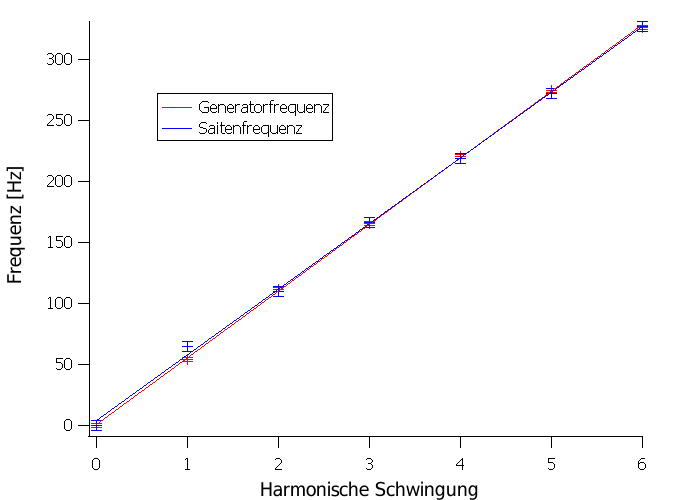
\includegraphics[width=0.5\textwidth]{Aufgabe1.png}
    \end{figure}}
\end{frame}

\subsection{Bildunterschrift}
\begin{frame}[fragile]
\frametitle{Bildunterschrift}
  \begin{semiverbatim}
    \uncover<1->{\\begin\{figure\}}
    \uncover<1->{  \\includegraphics[width=0.3\\textwidth]\{Aufgabe1.png\}}
    \uncover<1->{  \alert<2>{\\caption\{}Linearer Anstieg der Frequenz mit \(N\)\alert<2>{\}}}
    \uncover<1->{\\end\{figure\}}
  \end{semiverbatim}
  \uncover<3->{%
    \begin{figure}
      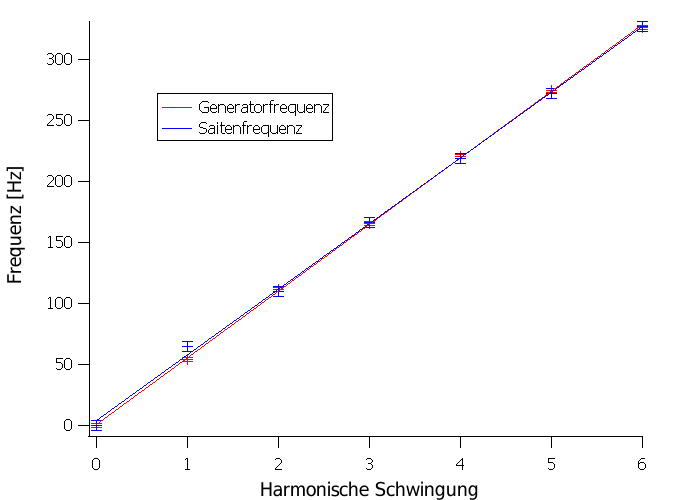
\includegraphics[width=0.3\textwidth]{Aufgabe1.png}
      \caption{Linearer Anstieg der Frequenz mit \(N\)}
    \end{figure}}
\end{frame}

\subsection{Positionierung von Abblidungen}
\begin{frame}[fragile]
\frametitle{Positionierung von Abbildungen}
  \begin{semiverbatim}
    \uncover<1->{\\begin\{figure\}\alert<1>{[htbp]}}
    \uncover<1->{  \\includegraphics[width=0.3\\textwidth]\{Aufgabe1.png\}}
    \uncover<1->{  \\caption\{Linearer Anstieg der Frequenz mit \(N\)\}}
    \uncover<1->{\\end\{figure\}}
  \end{semiverbatim}
  \begin{itemize}
    \item[h (here)]<3-> Positioniert bevorzugt an der Textstelle, an der die Umgebung steht
    \item[t (top)]<4-> Positioniert bevorzugt am Seitenanfang
    \item[b (bottom)]<5-> Positioniert bevorzugt am Seitenende
    \item[p (page)]<6-> Positioniert auf neuer Seite
    \item[H (HERE)]<7-> Mit Paket "`here"': erwzingt Position an dieser Stelle - kann zu Fehlern führen
  \end{itemize}
\end{frame}


 
\section{Quellenverzeichnis}
\begin{frame}
 \begin{center}
  \Huge Paket: bibtex 
 \end{center}
\end{frame}


\section{Referenzen}
\begin{frame}
 \begin{center}
  \Huge Referenzen/Querverweise
 \end{center}
\end{frame}

\begin{frame}[fragile]
\frametitle{Referenzen}
  \begin{itemize}
    \item[]<1-> Was kann alles referenziert werden?
    \begin{itemize}
      \item<2-> Abbildungen
      \item<3-> Tabellen
      \item<4-> Gliederungselemente(\verb+\part{}+,\verb+\section{}+,...)
      \item<5-> Formeln
      \item<6-> Aufzählungselemente
    \end{itemize}
    \item[]
    \item[]<7-> Was kann angezeigt werden?
    \begin{itemize}
      \item<8-> Nummer des Elements
      \item<9-> Nummer der Seite, auf der das Element steht 
    \end{itemize}
  \end{itemize}
\end{frame}

\subsection{Abbildungsreferenz}
\begin{frame}[fragile]
\frametitle{Refernzen auf Abbildungen}
  \begin{semiverbatim}
    \uncover<1->{\\begin\{figure\}[htbp]}
    \uncover<1->{  \\includegraphics[width=0.3\\textwidth]\{Aufgabe1.png\}}
    \uncover<1->{  \\caption\{Linearer Anstieg der Frequenz mit \(N\)\}}
    \uncover<2->{  \alert<2>{\\label\{frequenz\}}}
    \uncover<1->{\\end\{figure\}}
    \uncover<1->{}
    \uncover<1->{}
    \uncover<1->{}
    \uncover<3->{Die Abbildung \alert<3>{\\ref\{frequenz\}} \hspace{1cm} Die Abbildung 1}
    \uncover<4->{auf Seite \alert<4>{\\pageref\{frequenz\}} \hspace{1cm} auf Seite 6}
  \end{semiverbatim}
\end{frame}

\subsection{Abschnittsreferenz}
\begin{frame}[fragile]
\frametitle{Referenzen auf Abschnitte}
  \begin{semiverbatim}
    \uncover<1->{\\section\{Integration \\& Differentiation\}}
    \uncover<1->{  Wichtige Regeln für Integration und}
    \uncover<1->{  Differentiation}
    \uncover<1->{}
    \uncover<1->{  \\subsection\{Differentiation\}}
    \uncover<1->{  \alert<2>{\\label\{Diff\}}}
    \uncover<1->{}
    \uncover<1->{}
    \uncover<3->{In Abschnitt \alert<3>{\\ref\{Diff\}} \hspace{1cm} In Abschnitt 1.1}
    \uncover<4->{auf Seite \alert<4>{\\pageref\{Diff\}} \hspace{1cm} auf Seite 3}
  \end{semiverbatim}
\end{frame}

\subsection{Funktionenreferenz}
\begin{frame}[fragile]
\frametitle{Referenzen auf Funktionen}
  \begin{semiverbatim}
    \uncover<1->{\\begin\{align\}}
    \uncover<1->{  sin(\\alpha) = \\frac\{a\}\{c\}\\\\}
    \uncover<1->{  a^2 + b^2 = c^2 \alert<1>{\\label\{pyth\}}}
    \uncover<1->{\\end\{align\}}
    \uncover<1->{}
    \uncover<1->{}
    \uncover<1->{}
    \uncover<2->{wie Formel \alert<2>{\\ref\{pyth\}} \hspace{2cm} wie Formel 7}
    \uncover<3->{auf Seite \alert<3>{\\pageref\{pyth\}} \hspace{1cm} auf Seite 9}
  \end{semiverbatim}
\end{frame}

\subsection{Tabellenreferenzen}
\begin{frame}[fragile]
\frametitle{Referenz auf Tabellen}
  \begin{semiverbatim}
    \uncover<1->{\\begin\{table\}}
    \uncover<1->{  \\begin\{tabular\}\{|l|c|r|\}}
    \uncover<1->{    \\hline}
    \uncover<1->{    Tabelle & mit & drei Spalten \\\\ \\hline}
    \uncover<1->{    aber & nur mit zwei & Zeilen \\\\ \\hline}
    \uncover<1->{  \\end\{tabular\}}
    \uncover<1->{  \\caption\{Einfaches Tabellenbeispiel\}\alert<1>{\\label\{bsptab\}}}
    \uncover<1->{\\end\{table\}}
    \uncover<1->{}
    \uncover<1->{}
    \uncover<1->{}
    \uncover<2->{wie Tabelle \alert<2>{\\ref\{bsptab\}} \hspace{2cm} wie Tabelle 5}
    \uncover<2->{auf Seite \alert<2>{\\pageref\{bsptab\}} \hspace{1cm} auf Seite 97}
  \end{semiverbatim}
\end{frame}

\subsection{Referenzen auf Aufzählungselemente}
\begin{frame}[fragile]
\frametitle{Referenzen auf Aufzählungselemente}
  \begin{semiverbatim}
    \uncover<1->{\\begin\{enumerate\}}
    \uncover<1->{  \\item Zeichne L über p}
    \uncover<1->{  \\item Trage Fehlerkreuze ein \alert<1>{\\label\{fehler\}}}
    \uncover<1->{  \\item Konstruiere Fitgerade}
    \uncover<1->{\\end\{enumerate\}}
    \uncover<1->{}
    \uncover<1->{Aufgabe \alert<1>{\\ref\{fehler\}} ist nervig.}
  \end{semiverbatim}
  \uncover<2->{%
  \begin{enumerate}
    \item Zeichne L über p
    \item Trage Fehlerkreuze ein \label{fehler}
    \item Konstruiere Fitgerade
  \end{enumerate}
  Aufgabe \ref{fehler} ist nervig.}
\end{frame}


\section{ToDo-Paket}
\begin{frame}
 \begin{center}
  \Huge ToDo-Notizen
 \end{center}
\end{frame}

\subsection{Header und ToDo-Befehl}
\begin{frame}[fragile]
\frametitle{ToDo-Paket}
 \begin{semiverbatim}
	\uncover<1->{\small \\documentclass[a4paper,11pt,DIV=11,parskip=half*]\{scrartcl\}}
  \uncover<1->{\alert<1>{\\usepackage\{todonotes\}}}
  \uncover<1->{}
	\uncover<1->{\\begin\{document\}}
	\uncover<1->{}
	\uncover<2->{Hier muss noch etwas entstehen}
	\uncover<2->{\alert<2>{\\todo\{Ergebnisse zusammenfassen\}}}
	\uncover<1->{}
	\uncover<1->{\\end\{document\}}
 \end{semiverbatim}
 \uncover<3->{Hier muss noch etwas entstehen \todo{Ergebnisse zusammenfassen}}
\end{frame}

\subsection{Missing Figure}
\begin{frame}[fragile]
\frametitle{Fehlende Grafik}
 \begin{semiverbatim}
  \uncover<1->{\\begin\{figure\}}
  \uncover<2->{  \alert<2>{\\missingfigure\{NotizImBild\}}}
  \uncover<1->{  \\caption\{Bildunterschrift\}}
  \uncover<1->{\\end\{figure\}}
 \end{semiverbatim}
 \uncover<3->{%
  \begin{figure}
   \missingfigure{NotizImBild}
   \caption{Bildunterschrift}
  \end{figure}}
\end{frame}

\subsection{Übersicht über ToDo}
\begin{frame}[fragile]
\frametitle{Übersicht über ToDo-Liste}
 \begin{semiverbatim}
	\uncover<1->{\\maketitle}
  \uncover<1->{\\tableofcontents}
  \uncover<2->{\alert<2>{\\listoftodos}}
 \end{semiverbatim}
%  \uncover<3->{\listoftodos}
\end{frame}


\section{Präsentationen in Latex}
\begin{frame}
\frametitle{Präsentationen mit \LaTeX}
 \begin{center}
	\Huge Präsentationen in \LaTeX
 \end{center}
\end{frame}

\section{Header}
\begin{frame}[fragile]
\frametitle{Header}
  \begin{semiverbatim}
    \uncover<2->{\alert<2>{\\documentclass\{beamer\}}}
    \uncover<1->{}
    \uncover<2->{\alert<2>{\\mode<presentation>}}
    \uncover<1->{}
    \uncover<2->{\alert<2>{\\usetheme\{Montpellier\}}}
    \uncover<1->{\\usepackage[utf8]\{inputenc\}}
    \uncover<1->{\\usepackage[ngerman]\{babel\}}
    \uncover<1->{\\usepackage\{amsfonts,amsmath,amssymb\}}
    \uncover<1->{\\usepackage\{graphicx\}}
  \end{semiverbatim}
\end{frame}

\begin{frame}[fragile]
\frametitle{Header - Titeldaten}
  \begin{semiverbatim}
    \uncover<1->{\\title\{Präsentationen mit \\LaTeX\}}
    \uncover<2->{\alert<2>{\\subtitle\{eine kleine Einführung\}}}
    \uncover<1->{\\author\{Mein Name\}}
    \uncover<1->{\\date\{\\today oder Datum\}}
    \uncover<2->{\alert<2>{\\institute\{Universität Bremen, Fachbereich 1\}}}
  \end{semiverbatim}
\end{frame}

\section{Body}
\subsection{Titelseite und Gliederung}
\begin{frame}[fragile]
\frametitle{Dokument - Titelseite und Gliederung}
  \begin{semiverbatim}
    \uncover<1->{\\begin\{document\}}
    \uncover<2->{\\begin\{frame\}}
    \uncover<3->{  \\titlepage}
    \uncover<2->{\\end\{frame\}}
    \uncover<2->{}
    \uncover<4->{\\begin\{frame\}}
    \uncover<5->{  \\tableofcontents}
    \uncover<4->{\\end\{frame\}}
    \uncover<1->{\\end\{document\}}
  \end{semiverbatim}
\end{frame}

\subsection{Folien}
\begin{frame}[fragile]
\frametitle{Folien erstellen}
  \begin{semiverbatim}
    \uncover<1->{\\begin\{frame\}}
    \uncover<2->{\\frametitle\{Meine erste Folie\}}
    \uncover<3->{  \\begin\{itemize\}}
    \uncover<3->{    \\item \\LaTeX-Folien sind einfach}
    \uncover<3->{    \\item Struktur ist wichtig}
    \uncover<3->{    \\item Übersichtlich bleiben!}
    \uncover<3->{  \\end\{itemize\}}
    \uncover<1->{\\end\{frame\}}
  \end{semiverbatim}
\end{frame}

\begin{frame}
\frametitle{Meine erste Folie}
  \begin{itemize}
    \item \LaTeX-Folien sind einfach
    \item Struktur ist wichtig
    \item Übersichtlich bleiben!
  \end{itemize}
\end{frame}

\subsection{pause-Befehl}
\begin{frame}[fragile]
\frametitle{pause-Befehl}
  \begin{semiverbatim}
    \uncover<1->{\\begin\{frame\}}
    \uncover<1->{\\frametitle\{Meine erste Folie\}}
    \uncover<1->{  \\begin\{itemize\}}
    \uncover<1->{    \\item \\LaTeX-Folien sind einfach\alert<2->{\\pause}}
    \uncover<1->{    \\item Struktur ist wichtig\alert<2->{\\pause}}
    \uncover<1->{    \\item Übersichtlich bleiben}
    \uncover<1->{  \\end\{itemize\}}
    \uncover<1->{\\end\{frame\}}
  \end{semiverbatim}
\end{frame}

\begin{frame}
\frametitle{Meine erste Folie}
  \begin{itemize}
    \item \LaTeX-Folien sind einfach\pause
    \item Struktur ist wichtig\pause
    \item Übersichtlich bleiben
  \end{itemize}
\end{frame}

\subsection{Andere Möglichkeiten zu verzögern}
\begin{frame}[fragile]
\frametitle{andere Verzögerungsmöglichkeiten}
  \begin{semiverbatim}
    \uncover<1->{\\begin\{frame\}}
    \uncover<1->{\\frametitle\{Meine erste Folie\}}
    \uncover<1->{  \\begin\{itemize\}}
    \uncover<1->{    \\item\alert<2>{<1->} \\LaTeX-Folien sind einfach}
    \uncover<1->{    \\item\alert<2>{<3->} Struktur ist wichtig}
    \uncover<1->{    \\item\alert<2>{<2->} Übersichtlich bleiben}
    \uncover<1->{  \\end\{itemize\}}
    \uncover<1->{\\end\{frame\}}
  \end{semiverbatim}
\end{frame}

\begin{frame}
\frametitle{Meine erste Folie}
  \begin{itemize}
    \item<1-> \LaTeX-Folien sind einfach
    \item<3-> Struktur ist wichtig
    \item<2-> Übersichtlich bleiben
  \end{itemize}
\end{frame}

\subsection{Hervorheben}
\begin{frame}[fragile]
\frametitle{Hervorheben}
  \begin{semiverbatim}
    \uncover<1->{\\begin\{frame\}}
    \uncover<1->{\\frametitle\{Meine erste Folie\}}
    \uncover<1->{  \\begin\{itemize\}}
    \uncover<1->{    \\item \\LaTeX-Folien sind \alert<2->{\\alert<1-2>\{einfach\}}}
    \uncover<1->{    \\item \alert<2->{\\alert<-3>\{Struktur\}} ist wichtig}
    \uncover<1->{    \\item \alert<2->{\\alert<4>\{Übersichtlich\}} bleiben}
    \uncover<1->{  \\end\{itemize\}}
    \uncover<1->{\\end\{frame\}}
  \end{semiverbatim}
\end{frame}

\begin{frame}
\frametitle{Meine erste Folie}
  \begin{itemize}
    \item \LaTeX-Folien sind \alert<1-2>{einfach}
    \item \alert<-3>{Struktur} ist wichtig
    \item \alert<4>{Übersichtlich} bleiben
  \end{itemize}
\end{frame}

\subsection{Grafiken einbinden}
\begin{frame}[fragile]
\frametitle{Grafiken einbinden}
  \begin{semiverbatim}
    \uncover<1->{\\begin\{frame\}}
    \uncover<1->{\\frametitle\{Grafiken\}}
    \uncover<2->{  \\begin\{figure\}[htb]}
    \uncover<3->{    \\includegraphics[height=0.7\\textheight]\{Aufgabe1.png\}}
    \uncover<4->{    \\caption\{Aufgabe 1\}}
    \uncover<2->{  \\end\{figure\}}
    \uncover<1->{\\end\{frame\}}
  \end{semiverbatim}
\end{frame}

\begin{frame}
\frametitle{Grafiken einbinden}
  \begin{figure}[htb]
    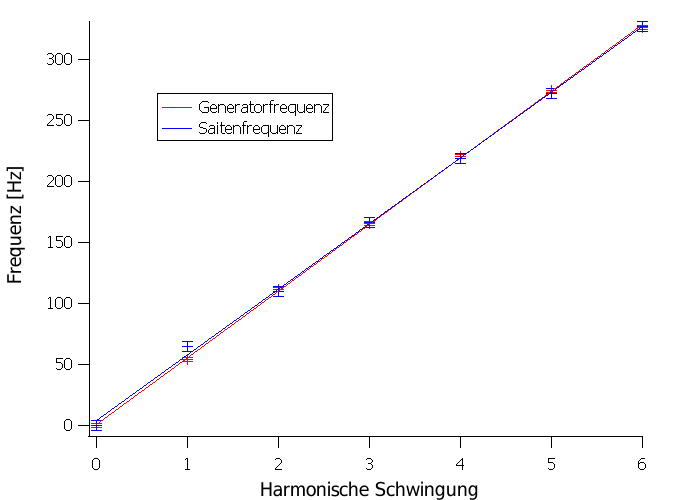
\includegraphics[height=0.7\textheight]{Aufgabe1.png}
    \caption{Aufgabe 1}
  \end{figure}
\end{frame}

\subsection{Seitenlayout}
\begin{frame}[fragile]
\frametitle{Seitenlayout}
  \begin{semiverbatim}
    \uncover<1->{\\begin\{frame\}}
    \uncover<1->{\\frametitle\{Geordnete Folie\}}
    \uncover<2->{  \\begin\{figure\}}
    \uncover<3->{    \\begin\{minipage\}\{0.49\\textwidth\}}
    \uncover<4->{      \\includegraphics[width=\\textwidth]\{Aufgabe1.png\}}
    \uncover<3->{    \\end\{minipage\}\\pause}
    \uncover<5->{    \\begin\{minipage\}\{0.49\\textwidth\}}
    \uncover<6->{      \\begin\{itemize\}}
    \uncover<7->{        \\item Diese Aufgabe ist sinnvoll}
    \uncover<6->{      \\end\{itemize\}}
    \uncover<5->{    \\end\{minipage\}}
    \uncover<2->{  \\end\{figure\}}
    \uncover<1->{\\end\{frame\}}
  \end{semiverbatim}
\end{frame}

\begin{frame}
\frametitle{Geordnete Folie}
  \begin{figure}
    \begin{minipage}{0.49\textwidth}
      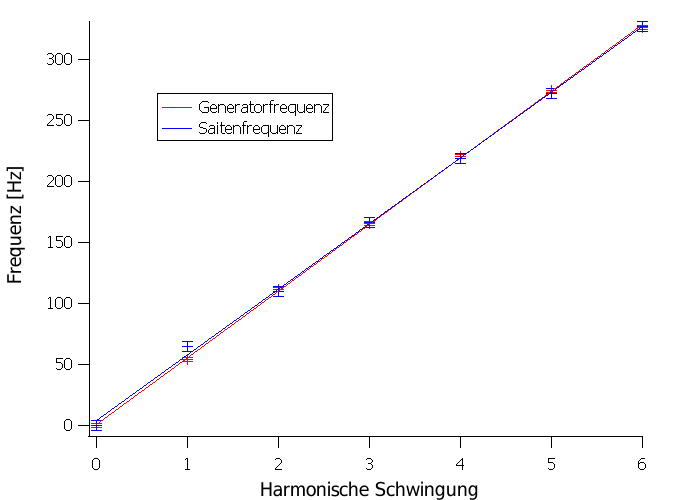
\includegraphics[width=\textwidth]{Aufgabe1.png}
    \end{minipage}\pause
    \begin{minipage}{0.49\textwidth}
      \begin{itemize}
	\item Diese Aufgabe ist sinnvoll
      \end{itemize}
    \end{minipage}
  \end{figure}
\end{frame}

\begin{frame}[fragile]
\frametitle{Seitenlayout}
  \begin{semiverbatim}
    \uncover<1->{\\begin\{frame\}}
    \uncover<1->{\\frametitle\{Geordnete Folie\}}
    \uncover<1->{  \\begin\{figure\}}
    \uncover<1->{    \alert<1>{\\uncover<2->\{\%}}
    \uncover<1->{    \\begin\{minipage\}\{0.49\\textwidth\}}
    \uncover<1->{      \\includegraphics[width=\\textwidth]\{Aufgabe1.png\}}
    \uncover<1->{    \\end\{minipage\}\alert<1>{\}}}
    \uncover<1->{    \alert<1>{\\uncover<1->\{\%}}
    \uncover<1->{    \\begin\{minipage\}\{0.49\\textwidth\}}
    \uncover<1->{      \\begin\{itemize\}}
    \uncover<1->{        \\item Dieser Graph soll später erscheinen}
    \uncover<1->{      \\end\{itemize\}}
    \uncover<1->{    \\end\{minipage\}\alert<1>{\}}}
    \uncover<1->{  \\end\{figure\}}
    \uncover<1->{\\end\{frame\}}
  \end{semiverbatim}
\end{frame}

\begin{frame}
\frametitle{Geordnete Folie}
  \begin{figure}
	 \uncover<2->{%
    \begin{minipage}{0.49\textwidth}
      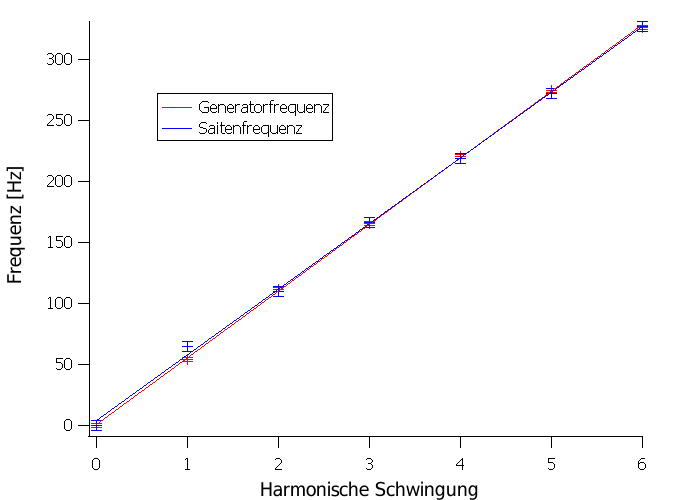
\includegraphics[width=\textwidth]{Aufgabe1.png}
    \end{minipage}}
	 \uncover<1->{%
    \begin{minipage}{0.49\textwidth}
      \begin{itemize}
	\item Dieser Graph soll später erscheinen
      \end{itemize}
    \end{minipage}}
  \end{figure}
\end{frame}

\section{Abgesang}
\subsection{Allgemeine Tipps für LaTeX}
\begin{frame}
\frametitle{Allgemeine Tipps für \LaTeX}
  \begin{itemize}
    \item<1-> Übung macht den Meister - also erstmal möglichst viel in TeX schreiben!
    \item<2-> Bei Fragen: fragt jemanden der das benutzt (Fachbereich 1-5) oder nutzt Google
    \item<3-> logisches Einrücken macht eure Datei übersichtlich
    \item<4-> Mit \% könnt ihr Zeilen auskommentieren
    \item<5-> Warnings und badboxes sind nicht unbedingt ein Problem - Fehler schon!
  \end{itemize}
\end{frame}

\begin{frame}
\frametitle{Fehlersuche in \LaTeX}
  \begin{itemize}
    \item<1-> Fehlermeldung lesen!
    \item<2-> Zeile des Fehlers in Umgebung $\rightarrow$ meist eine Klammer vergessen - \} oder \{
    \item<3-> Fehler in längerem Abschnitt: Alles mit \% auskommentieren und Stück für Stück wieder in den Text nehmen
    \item<4-> Hat jedes \alert<4>{begin} auch ein \alert<4>{end}?
    \item<5-> Fehlt evtl ein \alert<5>{usepackage}?
    \item<6-> Google zu dem Fehler befragen
  \end{itemize}
\end{frame}


\begin{frame}
 \Huge Aktuell noch Fragen?
\end{frame}

\subsection{Ende}
\begin{frame}
\Huge Viel Erfolg im ersten Semester!
\end{frame}

\end{document}









